\documentclass[tikz,border=0pt]{standalone}
\usepackage{fontspec}
\usepackage{tikz}
\usetikzlibrary{arrows.meta,calc}
\setmainfont[Path=C:/Windows/Fonts/,UprightFont=GOTHIC.TTF,BoldFont=GOTHICB.TTF,ItalicFont=GOTHICI.TTF,BoldItalicFont=GOTHICBI.TTF]{Century Gothic}
\definecolor{navy}{HTML}{0C171F}
\tikzset{
  box/.style={draw=navy,line width=0.9pt,rounded corners=4pt},
  focus/.style={draw=navy,line width=1.15pt,rounded corners=5pt},
  internal/.style={draw=navy,line width=0.9pt,rounded corners=6pt,dash pattern=on 5pt off 4pt},
  key/.style={text=navy,font=\bfseries\fontsize{10.5}{12.5}\selectfont,align=center},
  label/.style={text=navy,font=\fontsize{7.7}{9.4}\selectfont,align=center},
  small/.style={text=navy,font=\fontsize{6.9}{8.4}\selectfont,align=center},
  heading/.style={text=navy,font=\bfseries\fontsize{11.5}{13.5}\selectfont,anchor=west},
  arrow/.style={-{Latex[length=2.7mm,width=1.8mm]},draw=navy,line width=0.9pt},
  update/.style={-{Latex[length=2.7mm,width=1.8mm]},draw=navy,line width=0.95pt,rounded corners=5pt}
}
\begin{document}
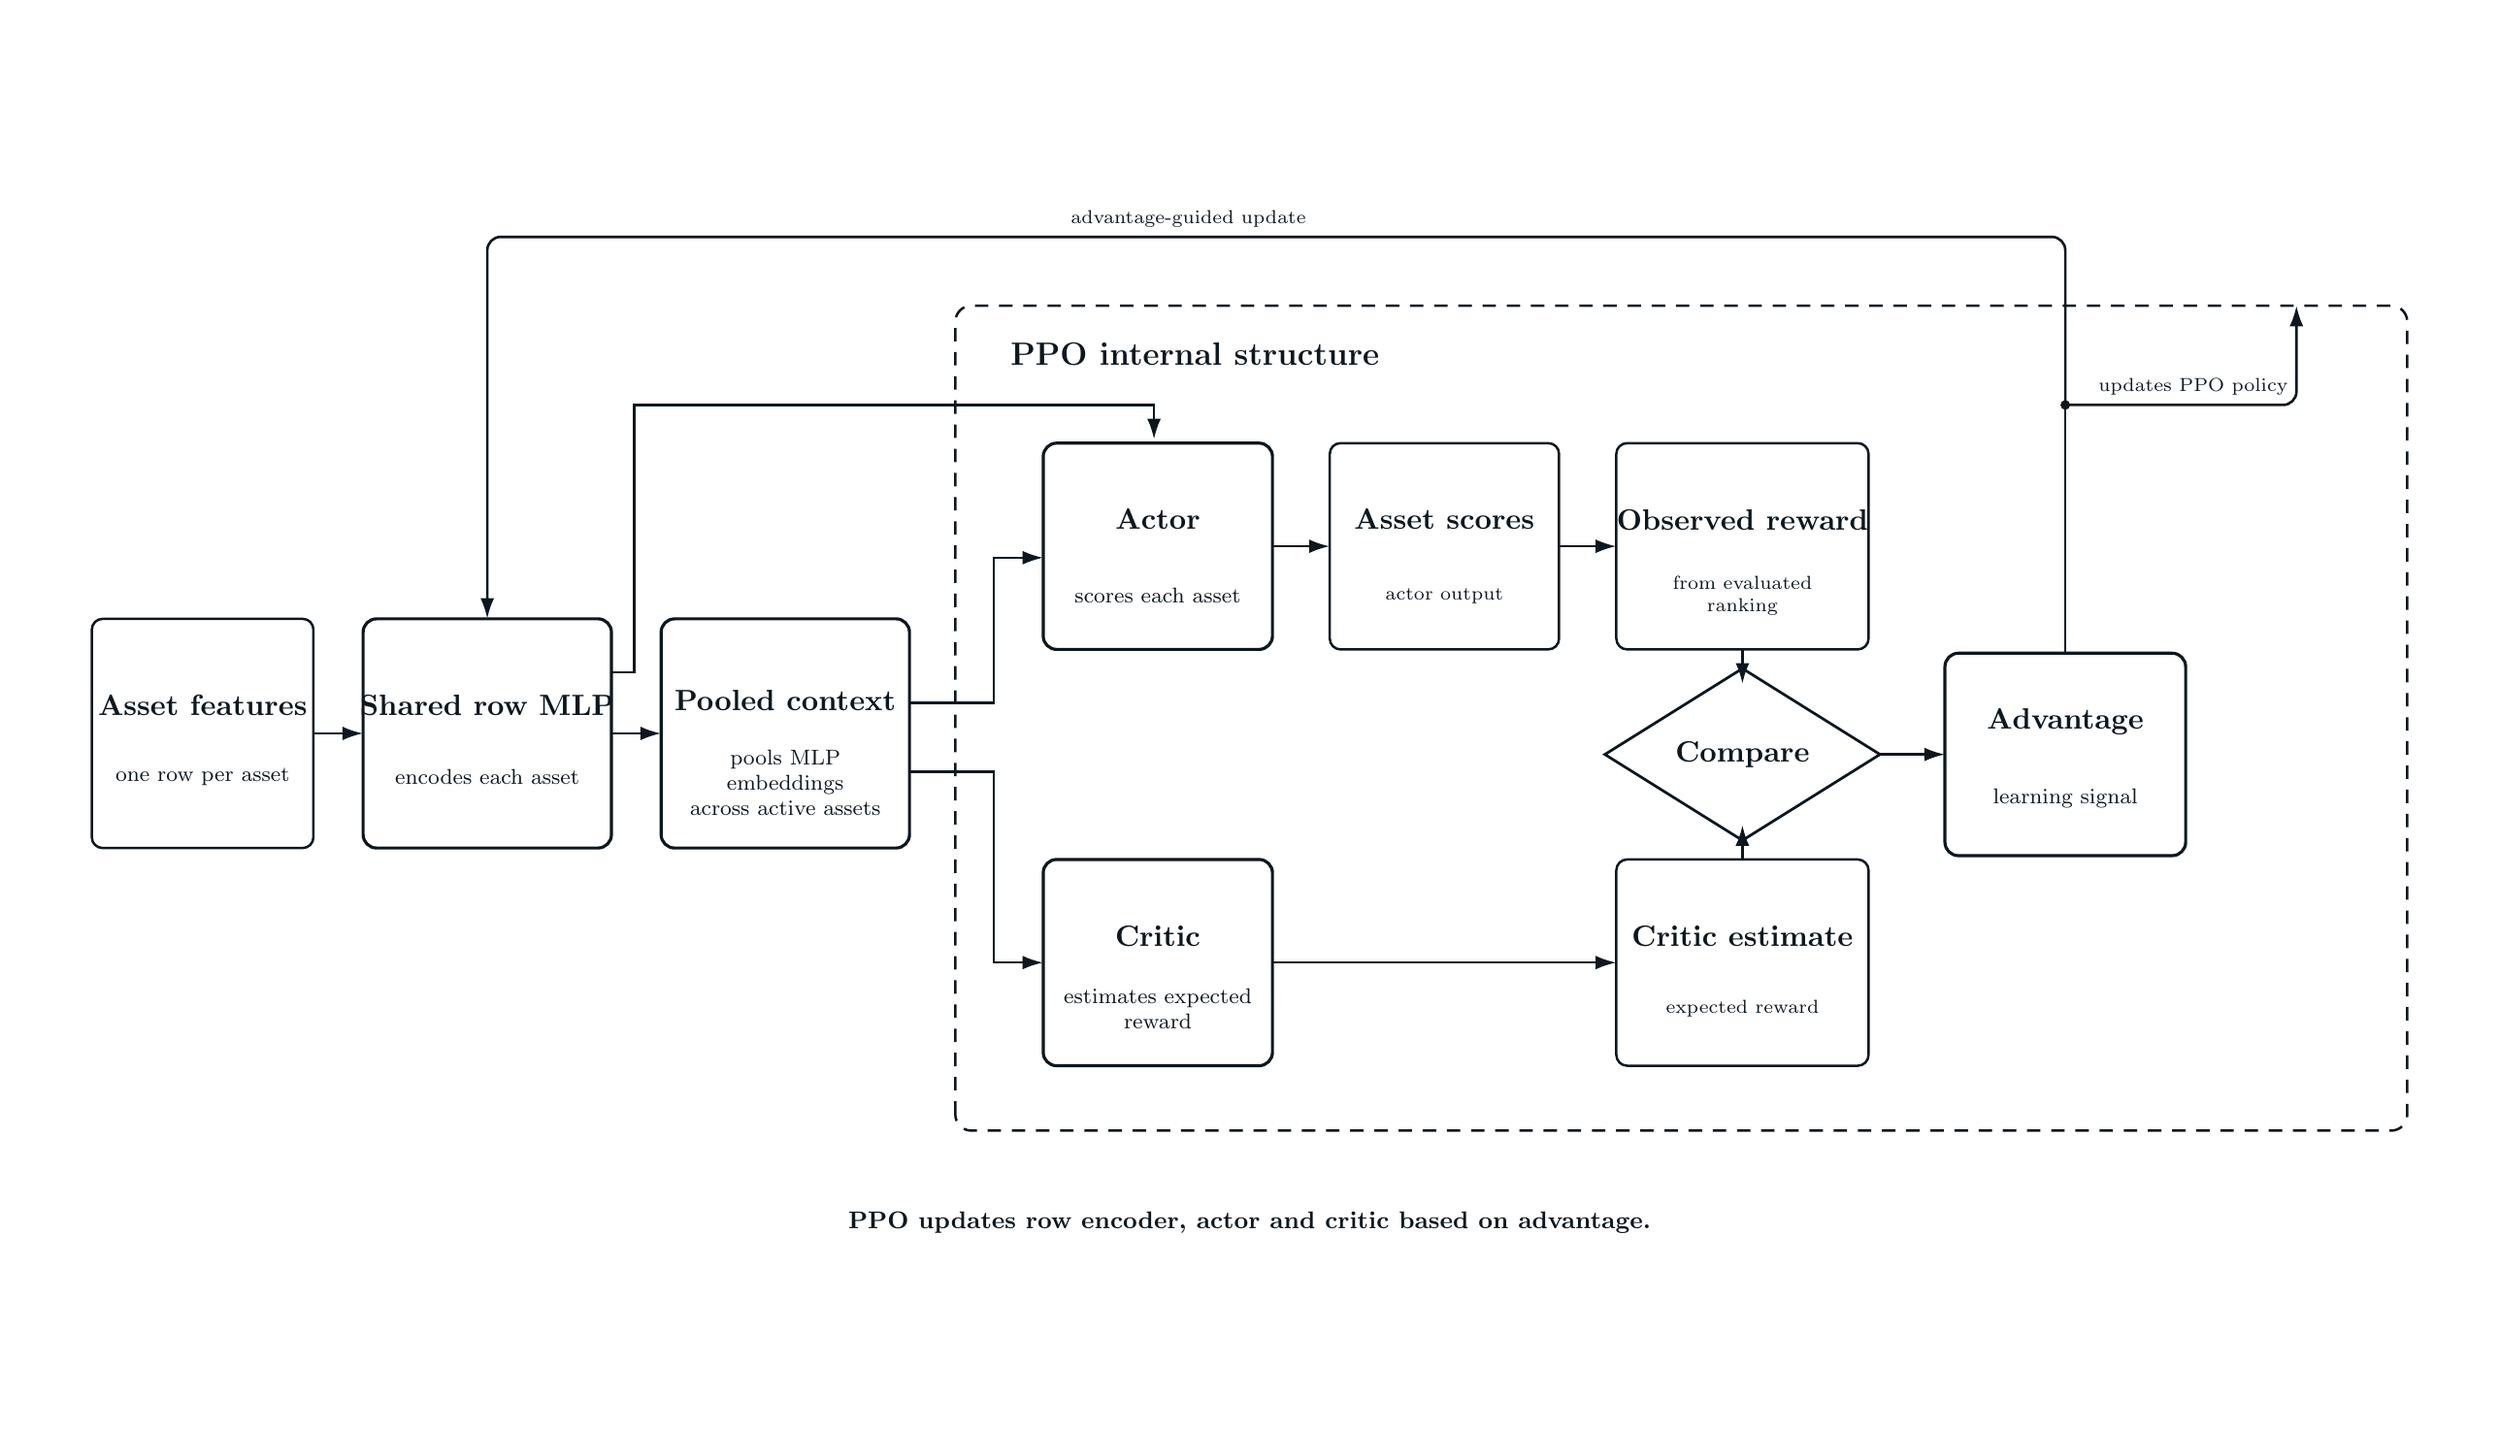
\begin{tikzpicture}[x=1cm,y=1cm]
  \path[use as bounding box] (0,0) rectangle (32,18);

  % Shared representation.
  \draw[box] (0.85,7.25) rectangle (3.75,10.25);
  \node[key] at (2.30,9.12) {Asset features};
  \node[label] at (2.30,8.18) {one row per asset};

  \draw[arrow] (3.75,8.75) -- (4.40,8.75);
  \draw[focus] (4.40,7.25) rectangle (7.65,10.25);
  \node[key] at (6.025,9.12) {Shared row MLP};
  \node[label] at (6.025,8.18) {encodes each asset};

  \draw[arrow] (7.65,8.75) -- (8.30,8.75);
  \draw[focus] (8.30,7.25) rectangle (11.55,10.25);
  \node[key] at (9.925,9.18) {Pooled context};
  \node[label,text width=2.70cm] at (9.925,8.10) {pools MLP embeddings\\across active assets};

  % PPO internals.
  \draw[internal] (12.15,3.55) rectangle (31.15,14.35);
  \node[heading] at (12.75,13.72) {PPO internal structure};

  % Actor: direct row embeddings plus pooled context.
  \draw[arrow] (7.65,9.55) -- (7.95,9.55) -- (7.95,13.05) -- (14.75,13.05) -- (14.75,12.60);
  \draw[arrow] (11.55,9.15) -- (12.65,9.15) -- (12.65,11.05) -- (13.30,11.05);
  \draw[focus] (13.30,9.85) rectangle (16.30,12.55);
  \node[key] at (14.80,11.55) {Actor};
  \node[label] at (14.80,10.55) {scores each asset};

  \draw[arrow] (16.30,11.20) -- (17.05,11.20);
  \draw[box] (17.05,9.85) rectangle (20.05,12.55);
  \node[key] at (18.55,11.55) {Asset scores};
  \node[small] at (18.55,10.55) {actor output};

  \draw[arrow] (20.05,11.20) -- (20.80,11.20);
  \draw[box] (20.80,9.85) rectangle (24.10,12.55);
  \node[key] at (22.45,11.55) {Observed reward};
  \node[small] at (22.45,10.55) {from evaluated\\ranking};

  % Critic: pooled summary derived from MLP embeddings.
  \draw[arrow] (11.55,8.25) -- (12.65,8.25) -- (12.65,5.75) -- (13.30,5.75);
  \draw[focus] (13.30,4.40) rectangle (16.30,7.10);
  \node[key] at (14.80,6.10) {Critic};
  \node[label] at (14.80,5.15) {estimates expected\\reward};

  \draw[arrow] (16.30,5.75) -- (20.80,5.75);
  \draw[box] (20.80,4.40) rectangle (24.10,7.10);
  \node[key] at (22.45,6.10) {Critic estimate};
  \node[small] at (22.45,5.15) {expected reward};

  % Spacious, symmetric comparison.
  \draw[arrow] (22.45,9.85) -- (22.45,9.40);
  \draw[arrow] (22.45,7.10) -- (22.45,7.55);
  \draw[navy,line width=1pt] (22.45,7.35) -- (24.25,8.475) -- (22.45,9.60) -- (20.65,8.475) -- cycle;
  \node[key] at (22.45,8.475) {Compare};

  \draw[arrow] (24.25,8.475) -- (25.10,8.475);
  \draw[focus] (25.10,7.15) rectangle (28.25,9.80);
  \node[key] at (26.675,8.90) {Advantage};
  \node[label] at (26.675,7.90) {learning signal};

  % One advantage branch updates PPO policy and the shared encoder.
  \draw[navy,line width=0.95pt] (26.675,9.80) -- (26.675,13.05);
  \fill[navy] (26.675,13.05) circle (1.8pt);
  \draw[update] (26.675,13.05) -- (29.70,13.05) -- (29.70,14.35);
  \node[small,anchor=south] at (28.35,13.05) {updates PPO policy};
  \draw[update] (26.675,13.05) -- (26.675,15.25) -- (6.025,15.25) -- (6.025,10.25);
  \node[small,anchor=south] at (15.20,15.25) {advantage-guided update};

  \node[text=navy,font=\bfseries\fontsize{9.2}{11.2}\selectfont,align=center] at (16,2.35)
    {PPO updates row encoder, actor and critic based on advantage.};
\end{tikzpicture}
\end{document}
